\begin{figure}[t]
    \centering
    \includegraphics[width=0.8\columnwidth]{Image/graphs/sampling_method.pdf}
    \caption{These graphs display changes in error rates as the sampling rate increases for three different sampling strategies in the $Lucy$ benchmark with a 0.5 overlap ratio.}
    \label{fig_sampling_method}
\end{figure}
%
%
\Skip{
\begin{figure}[t]
    \centering
    \begin{subfigure}[b]{0.9\linewidth}
        \centering
       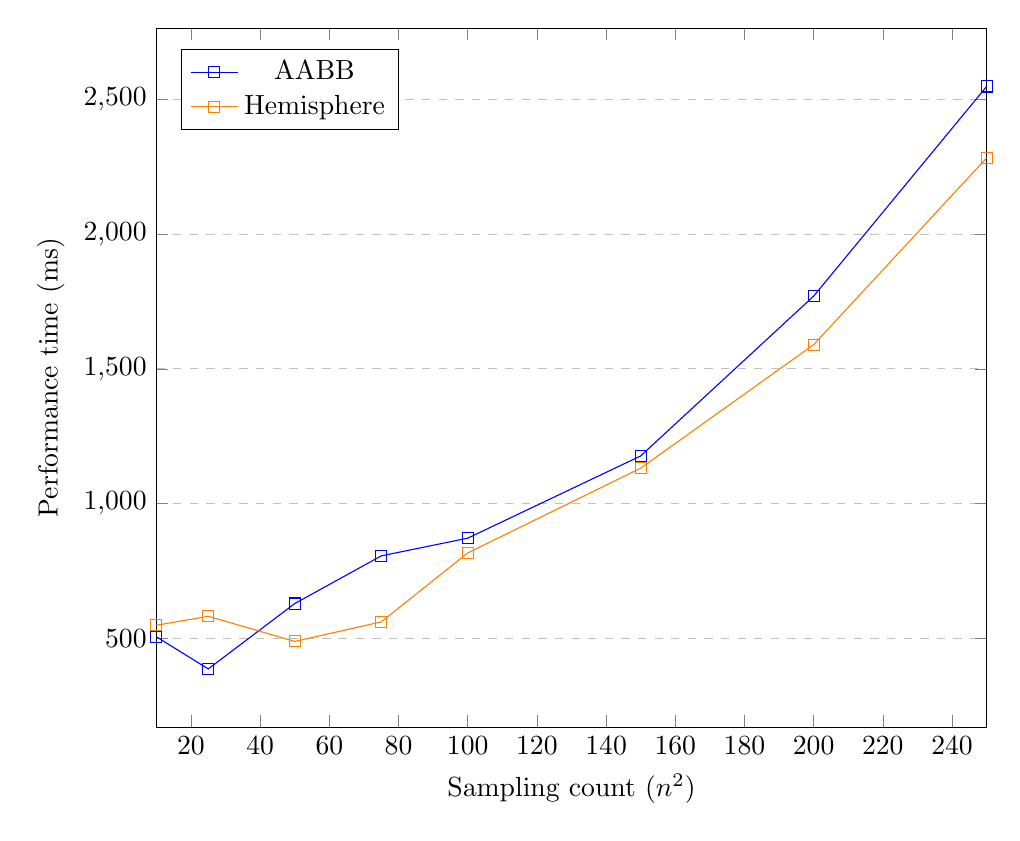
\begin{tikzpicture}
    \begin{axis}[
    width=\linewidth,
    xlabel={Sampling count ($n^2$)},
    ylabel={Performance time (ms)},
    xmin=10,
    xmax=250,
    legend pos=north west,
    ymajorgrids=true,
    grid style=dashed,
]
\addplot[color=blue, mark=square] coordinates {(10, 506.68)(25, 387.56)(50,629.92)(75,806.73)(100,872.39)(150,1177.29)(200,1769.80)(250,2547.22)};
\addplot[color=orange, mark=square] coordinates {(10, 549.48)(25, 582.76)(50,489.61)(75,561.96)(100,817.6)(150,1131.89)(200,1589.88)(250,2282.16)}; \legend{AABB,Hemisphere}
    \end{axis}
\end{tikzpicture}
        \caption{Performance time (ms)}
        \label{fig:graph_compare_sampling_method_performance_time}
    \end{subfigure}
    \hfill
    \begin{subfigure}[b]{0.9\linewidth}
        \centering
        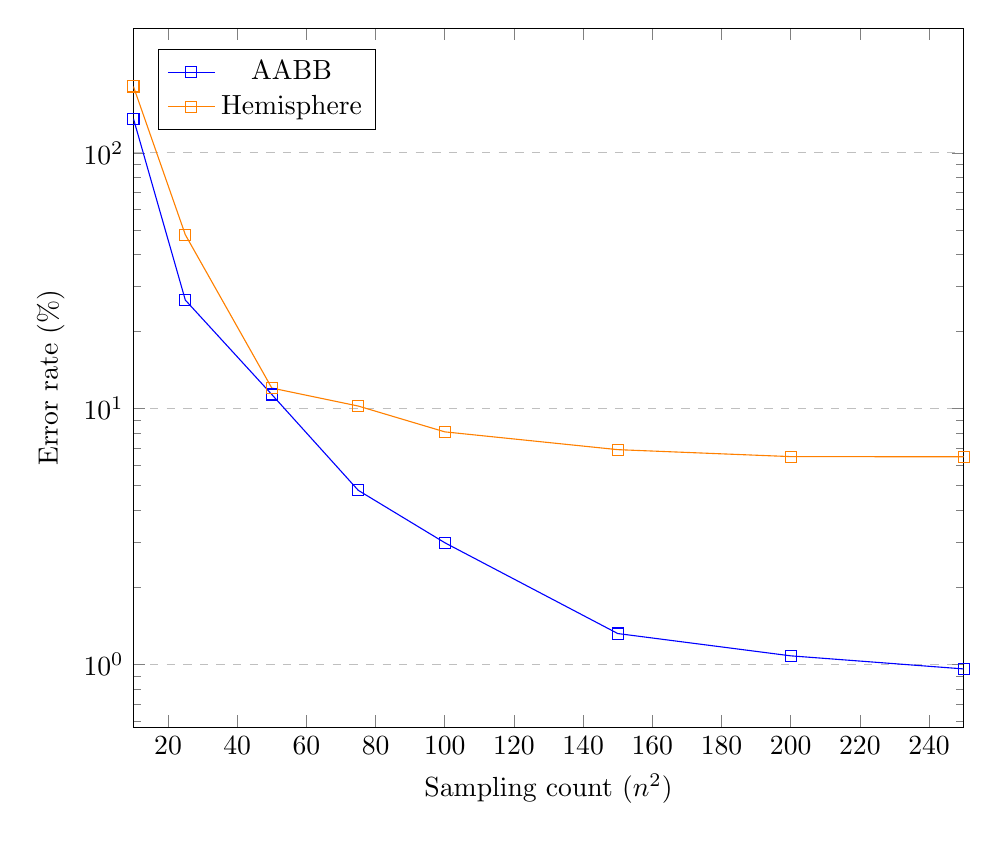
\begin{tikzpicture}
    \begin{axis}[
    width=\linewidth,
    xlabel={Sampling count ($n^2$)},
    ylabel={Error rate (\%)},
    xmin=10,
    xmax=250,
    legend pos=north west,
    ymajorgrids=true,
    grid style=dashed,
    ymode = log,
]
%\addplot[color=red, mark=square] coordinates {(10, 0.01)(25, 0.01)(50,0.01)(75,0.01)(100,0.01)(150,0.01)(200,0.01)(250,0.01)};
\addplot[color=blue, mark=square] coordinates {(10, 135.95)(25, 26.56)(50,11.35)(75,4.79)(100,2.99)(150,1.32)(200,1.08)(250,0.96)};
\addplot[color=orange, mark=square] coordinates {(10, 181.68)(25, 47.82)(50,12.03)(75,10.23)(100,8.11)(150,6.91)(200,6.49)(250,6.48)}; \legend{AABB,Hemisphere}
    \end{axis}
\end{tikzpicture}
        \caption{Error rate (\%)}\label{fig:graph_compare_sampling_method_error_rate}
    \end{subfigure}
    \caption{Compare the results of each sampling method according to the number of samples.
    }
    \label{fig:comparison_sampling_methods}
\end{figure}
}